
\begin{figure}
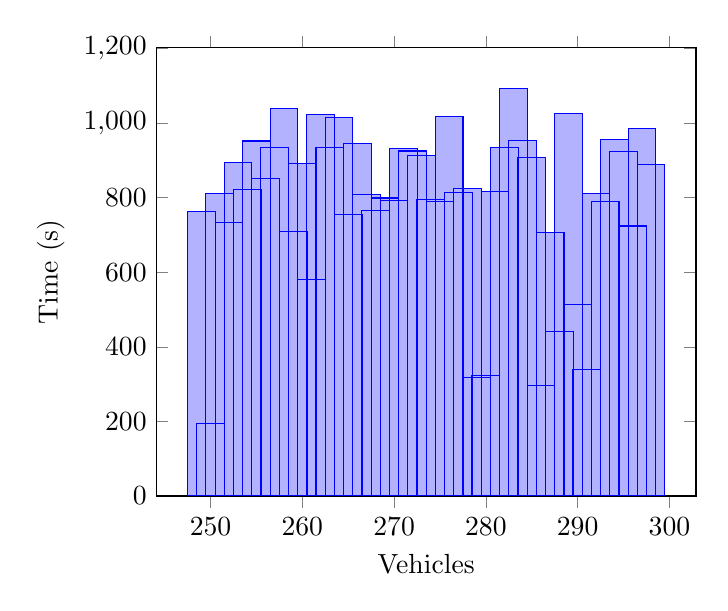
\begin{tikzpicture}
\begin{axis}[
legend style={anchor=west},
xlabel=Vehicles,
ylabel=Time (s),
ymin=0,
ybar,
]
\addplot coordinates {
(297, 986)
(294, 956)
(281, 817)
(287, 707)
(250, 195)
(283, 1093)
(253, 894)
(270, 793)
(288, 442)
(261, 581)
(293, 789)
(275, 789)
(255, 952)
(285, 908)
(292, 812)
(290, 514)
(262, 1023)
(291, 340)
(249, 762)
(289, 1025)
(251, 812)
(260, 892)
(258, 1040)
(271, 933)
(295, 924)
(298, 890)
(278, 824)
(277, 815)
(252, 734)
(268, 765)
(279, 317)
(280, 323)
(284, 954)
(272, 925)
(273, 912)
(269, 799)
(274, 795)
(267, 808)
(259, 709)
(257, 935)
(266, 945)
(256, 851)
(276, 1018)
(254, 822)
(263, 934)
(264, 1014)
(286, 296)
(282, 935)
(296, 724)
(265, 756)
};

\end{axis}
\end{tikzpicture}
\label{tik:time:0:90}
\caption{0 percent diving with GSC on route $90$}
\end{figure}
